% =====================================================================
% TA-IND-01 -- Informe Academico Individual
% Analisis Critico de un Sistema Distribuido Real: Apache Kafka (KRaft)
% Compilacion: pdflatex -> biber -> pdflatex -> pdflatex
% =====================================================================
\documentclass[11pt,a4paper]{article}

\usepackage[utf8]{inputenc}
\usepackage[T1]{fontenc}
\usepackage{lmodern}
\usepackage[spanish,es-tabla,es-nodecimaldot]{babel}
\usepackage{csquotes}
\usepackage[a4paper,top=2.5cm,bottom=2.5cm,left=2.5cm,right=2.5cm]{geometry}
\usepackage{graphicx}
\usepackage{booktabs}
\usepackage{float}
\usepackage{array}
\usepackage{amsmath}
\usepackage{setspace}
\usepackage{xurl}
\usepackage[backend=biber,style=ieee]{biblatex}
\addbibresource{referencias.bib}
\usepackage[hidelinks]{hyperref}

\setstretch{1.15}
\setlength{\parskip}{0.4em}

\begin{document}

% =====================================================================
% 1. CARATULA
% =====================================================================
\begin{titlepage}
\thispagestyle{empty}
\centering
{\Large\bfseries Universidad Técnica Estatal de Quevedo (UTEQ)\par}
\vspace{0.3cm}
{\large Facultad de Ciencias de la Computación (FCC)\par}
\vspace{0.2cm}
{\large Carrera de Ingeniería de Software\par}
\vspace{1.8cm}
{\large Asignatura: Sistemas Distribuidos (7mo Nivel / Semestre)\par}
\vspace{1.5cm}
{\large\bfseries TA-IND-01 --- Informe Académico Individual:\par}
\vspace{0.2cm}
{\large\bfseries Análisis Crítico de un Sistema Distribuido Real\par}
\vspace{1cm}
\rule{0.85\textwidth}{0.4pt}\par
\vspace{0.4cm}
{\LARGE\bfseries Apache Kafka en modo KRaft:\\[0.2cm]
transparencias, CAP/PACELC, comunicación y tolerancia a fallos\par}
\vspace{0.4cm}
\rule{0.85\textwidth}{0.4pt}\par
\vfill
\begin{tabular}{>{\bfseries}r l}
Estudiante: & Kenny Isaías España Vera \\[0.15cm]
Paralelo:   & 7mo SOFTWARE A \\[0.15cm]
Fecha:      & 13 de noviembre de 2026 \\
\end{tabular}
\vspace{1.2cm}

{\bfseries Repositorio GitHub:}\par
\vspace{0.15cm}
{\small\url{https://github.com/Luispaca2002/TA-IND-01-Informe-Acad-mico-Individual-An-lisis-Cr-tico-de-Sistemas-Distribuidos-Unidad-1-.git}\par}
\vspace{1cm}
{\large Quevedo -- Ecuador\par}
\end{titlepage}

% =====================================================================
% 2. RESUMEN
% =====================================================================
\newpage
\thispagestyle{empty}
\section*{Resumen}

Este informe analiza Apache Kafka, una plataforma de streaming de eventos basada en un log particionado y replicado, en su modo KRaft, que sustituye a ZooKeeper por un quórum de controladores basado en Raft. El análisis aplica los conceptos de la Unidad 1: transparencias de distribución, teorema CAP y su extensión PACELC, modelos de comunicación y tolerancia a fallos. Se contrastaron seis artículos científicos con documentación oficial, un incidente de producción documentado y un clúster propio de tres nodos desplegado con Docker Compose. Los resultados muestran que Kafka no es CP ni AP por naturaleza: con \texttt{acks=all}, \texttt{min.insync.replicas=2} y elección no limpia deshabilitada se comporta como PC/EC, rechazando escrituras antes que perder datos confirmados y pagando latencia de replicación en operación normal. Al detener un nodo, el clúster reeligió líderes y conservó el quórum, pero el cliente que usaba ese nodo como punto de arranque falló, lo que evidencia que la transparencia de fallos termina en el borde del cliente. Frente a RabbitMQ, Kafka gana en retención y paralelismo por partición, pero pierde en enrutamiento flexible y simplicidad operativa.

\vspace{0.4cm}
\noindent\textbf{Palabras clave:} Apache Kafka, KRaft, teorema CAP, PACELC, tolerancia a fallos, RabbitMQ.

\newpage
\setcounter{page}{1}
% La numeracion de secciones arranca en 3 para coincidir con la
% estructura de 13 secciones de la rubrica (1 = Caratula, 2 = Resumen).
\setcounter{section}{2}

% =====================================================================
% 3. INTRODUCCION
% =====================================================================
\section{Introducción}

Una cola de mensajes tradicional resuelve un problema concreto: desacoplar a quien produce un trabajo de quien lo ejecuta. El broker guarda el mensaje hasta que un consumidor lo confirma y luego lo elimina. Ese modelo funciona bien para distribuir tareas, pero se vuelve limitante cuando el mismo flujo de datos debe alimentar a varios sistemas con ritmos distintos, cuando se necesita volver a procesar eventos pasados o cuando el volumen obliga a repartir la carga entre muchas máquinas. Apache Kafka aborda ese escenario con otra abstracción: un log de solo escritura al final (\emph{append-only}), dividido en particiones, donde cada mensaje recibe un desplazamiento (\emph{offset}) secuencial y permanece almacenado según una política de retención, sin importar si ya fue leído \cite{raptis2023survey,kafkadocs}. El consumidor, no el broker, lleva la cuenta de por dónde va.

La adopción industrial confirma que el modelo escala. Raptis y Passarella, en una revisión sistemática de unos 70 trabajos, describen a Kafka como una plataforma ampliamente usada para streaming en red, con LinkedIn como caso de referencia \cite{raptis2023survey}. La propia LinkedIn reportó en 2019 más de 100 clústeres, más de 4000 brokers, más de 100\,000 topics, 7 millones de particiones y más de 7 billones (\emph{trillions}) de mensajes diarios \cite{linkedin2019}. Conviene leer esa cifra con cautela: es un dato autorreportado por la empresa que creó Kafka, no una medición auditada, y tiene varios años. Aun así, da una idea del orden de magnitud. En la literatura revisada para este informe, Kafka aparece en manufactura en la nube \cite{pacella2025scalable}, monitoreo de presión de aire en tiempo real \cite{zhou2024distributed}, gestión de datos industriales con OPC UA \cite{lu2025proposal} y plataformas IoT monitoreadas con Elastic Stack \cite{calderon2024monitoring}.

Elegí Kafka por una razón técnica precisa: es uno de los pocos sistemas en los que los compromisos que estudia la Unidad~1 no están ocultos en el diseño, sino expuestos como parámetros. Con \texttt{acks}, \texttt{min.insync.replicas} y \texttt{unclean.leader.election.enable}, el operador decide cuánta consistencia, disponibilidad y latencia quiere en cada topic \cite{kafkadocs}. Además, el sistema acaba de completar un cambio arquitectónico de fondo: la versión 4.0, publicada el 18 de marzo de 2025, es la primera que funciona sin ZooKeeper y depende por completo del quórum KRaft \cite{kafka40release}. Analizar Kafka hoy implica analizar ese nuevo plano de control.

El informe combina tres fuentes de evidencia: seis artículos científicos revisados y subrayados (Anexo~B), documentación oficial y un incidente real de producción, y un clúster de tres nodos en modo KRaft que desplegué localmente para observar la replicación y el comportamiento ante la caída de un nodo.

% =====================================================================
% 4. ARQUITECTURA DEL SISTEMA
% =====================================================================
\section{Arquitectura del sistema}
\label{sec:arquitectura}

\subsection{Productores}

Un productor publica registros formados por una clave y un valor en un topic \cite{raptis2023survey}. La clave determina la partición de destino: el particionador por defecto aplica un hash sobre la clave, de modo que todos los registros con la misma clave caen en la misma partición y conservan su orden relativo \cite{kafkadocs}. Esta decisión de diseño tiene una consecuencia directa: Kafka garantiza orden por partición, no por topic. El productor también agrupa registros en lotes y puede comprimirlos. Lu et al. compararon gzip, lz4 y snappy sobre mensajes JSON de 520 a 600 bytes y eligieron lz4 por su equilibrio entre tasa de compresión y velocidad, una elección adecuada para procesamiento sensible a la latencia \cite{lu2025proposal}.

\subsection{Brokers, topics y particiones}

Un clúster está formado por varios brokers, y las particiones de un mismo topic se distribuyen entre ellos \cite{zhou2024distributed}. La partición es la unidad básica de paralelismo: es una secuencia ordenada de mensajes en la que cada nuevo registro se agrega al final y recibe un offset secuencial \cite{raptis2023survey}. Cada partición se replica según un factor de replicación $RF$. Una réplica actúa como líder y atiende las lecturas y escrituras de esa partición; las demás son seguidoras que copian al líder y lo reemplazan si falla \cite{raptis2023survey}. Con $P$ particiones y $RF$ réplicas, el clúster aloja $P \times RF$ réplicas en total, repartidas entre los brokers.

\subsection{Segmentos de log}

En disco, cada partición no es un único archivo sino una secuencia de segmentos. Solo el segmento activo recibe escrituras; cuando alcanza un tamaño o una antigüedad configurados, se cierra y se abre uno nuevo \cite{kafkadocs}. La retención trabaja sobre segmentos completos: al vencer el plazo o superar el tamaño máximo, se eliminan segmentos enteros, lo que es mucho más barato que borrar mensajes individuales. Este diseño explica por qué Kafka puede retener días de datos sin degradar las escrituras: todas las operaciones de escritura son anexos secuenciales y las lecturas por offset se resuelven ubicando el segmento cuyo offset base es el inmediato inferior.

\subsection{Grupos de consumidores}

Los consumidores se organizan en grupos. Dentro de un grupo, cada partición se asigna a un único consumidor, lo que reparte la carga sin que dos miembros procesen el mismo mensaje \cite{raptis2023survey,kafkadocs}. De ahí sale un límite que conviene tener presente al dimensionar:
\begin{equation}
C_{\text{activos}} = \min(C, P),
\end{equation}
donde $C$ es el número de consumidores del grupo y $P$ el número de particiones. Un cuarto consumidor sobre un topic de tres particiones queda ocioso. Los offsets confirmados por cada grupo se guardan en un topic interno, \texttt{\_\_consumer\_offsets}, administrado por un coordinador de grupo \cite{kafkadocs}. La literatura revisada contiene aquí una imprecisión: Lu et al. afirman que KRaft registra el offset de cada mensaje y que el consumidor lo busca ahí \cite{lu2025proposal}. KRaft gestiona los metadatos del clúster (brokers, topics, particiones, líderes); los offsets de consumo viven en \texttt{\_\_consumer\_offsets} y la posición de cada registro es intrínseca al log de la partición \cite{kip500,kafkadocs}.

\subsection{De ZooKeeper al consenso interno KRaft}

Hasta la serie 3.x, Kafka dependía de ZooKeeper para almacenar los metadatos del clúster y coordinar la asignación de particiones y la recuperación ante fallos \cite{zhou2024distributed,calderon2024monitoring}. Uno de los brokers actuaba como controlador y, cada vez que se elegía uno nuevo, debía cargar el estado desde ZooKeeper antes de poder operar \cite{kip500}. Esto implicaba operar dos sistemas distribuidos distintos, con sus propios mecanismos de seguridad, monitoreo y fallo, y añadía tiempo a cada conmutación de controlador.

KIP-500 propuso reemplazar ZooKeeper por un quórum de controladores que gestiona un log de metadatos replicado mediante Raft; el líder de ese log es el controlador activo \cite{kip500}. Raft descompone el consenso en elección de líder, replicación del log y seguridad, y usa temporizadores aleatorios para resolver las elecciones \cite{ongaro2014raft}. Como cualquier protocolo de mayoría, un quórum de $N$ votantes tolera
\begin{equation}
f = \left\lfloor \frac{N-1}{2} \right\rfloor
\label{eq:quorum}
\end{equation}
fallos simultáneos. Con $N=3$ se tolera un fallo; con $N=5$, dos. La ventaja práctica es que los controladores seguidores ya tienen los metadatos replicados en memoria, por lo que la conmutación no exige recargar el estado desde un sistema externo \cite{kip500}. La versión 4.0 eliminó por completo el modo ZooKeeper \cite{kafka40release}. Lu et al. ya desplegaron su marco industrial con tres brokers gestionados por KRaft sobre Kafka 3.7.0 \cite{lu2025proposal}, mientras que Zhou et al. y Pacella et al. todavía trabajaron con ZooKeeper \cite{zhou2024distributed,pacella2025scalable}.

\subsection{Diagrama de arquitectura}
\label{sec:diagrama}

La Figura~\ref{fig:arquitectura} resume la arquitectura analizada.

\begin{figure}[H]
\centering
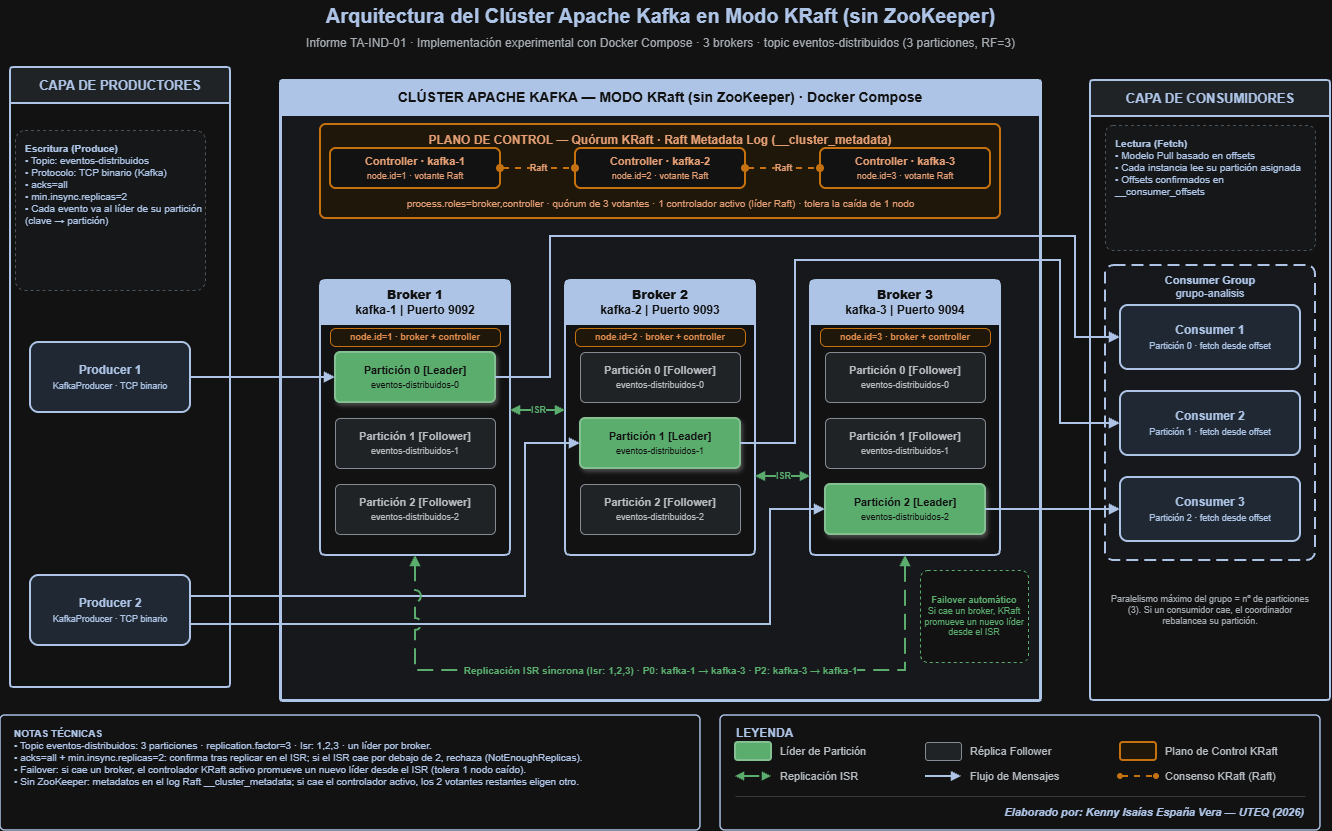
\includegraphics[width=0.92\textwidth]{evidencias/arquitectura_kafka.drawio.png}
\caption{Arquitectura de Apache Kafka en modo KRaft: productores, quórum de controladores, brokers con particiones líder y seguidoras, y grupos de consumidores. Elaboración propia a partir del esquema del Anexo~A.}
\label{fig:arquitectura}
\end{figure}

El diagrama parte del bosquejo dibujado a mano del Anexo~A. En esa primera versión ubiqué los componentes que reconocía en la lectura inicial: productores, un bloque de brokers y consumidores, con flechas de envío y lectura. Al contrastarlo con la documentación y con los artículos, el esquema resultó insuficiente en tres puntos. Primero, no distinguía el plano de control del plano de datos; en la versión limpia el quórum de controladores KRaft aparece separado del flujo de mensajes, porque su función es mantener metadatos y no transportar registros. Segundo, trataba al broker como unidad de almacenamiento, cuando la unidad real es la partición; por eso el diagrama final muestra particiones con su réplica líder y sus seguidoras repartidas entre nodos. Tercero, las flechas del bosquejo sugerían que el broker empuja mensajes al consumidor; el diagrama corregido invierte esa dirección para reflejar que el consumidor solicita lotes a partir de su offset \cite{raptis2023survey,kafkadocs}. Este último error es instructivo: el propio artículo de Raptis y Passarella menciona que Kafka admite consumo push y pull, aunque su ejemplo detallado describe un modelo pull \cite{raptis2023survey}; la documentación oficial justifica explícitamente el diseño pull \cite{kafkadocs}.

% =====================================================================
% 5. ANALISIS CON LOS CONCEPTOS DE LA UNIDAD 1
% =====================================================================
\section{Análisis con los conceptos de la Unidad 1}

\subsection{Transparencias de distribución}
\label{sec:transparencias}

Van Steen y Tanenbaum definen la transparencia de distribución como la capacidad de ocultar al usuario que procesos y recursos están repartidos en varias máquinas, y advierten que la transparencia total no siempre es deseable ni alcanzable \cite{vansteen2023distributed}. Kafka es un buen ejemplo de esa advertencia: oculta lo que puede ocultar sin costo y expone lo que, si se ocultara, impediría al cliente tomar decisiones correctas.

\textbf{Acceso.} Garantizada. Todos los clientes usan el mismo protocolo binario propio sobre TCP, independientemente del broker o del sistema operativo del servidor \cite{calderon2024monitoring,kafkadocs}. Un productor en Python y un consumidor en Java ven el mismo topic con la misma semántica.

\textbf{Ubicación.} Parcial. El cliente no necesita saber en qué broker reside cada partición: recibe una lista de servidores de arranque (\emph{bootstrap servers}), pide los metadatos y a partir de ellos se conecta directamente al líder de cada partición \cite{kafkadocs}. Sin embargo, la ubicación se filtra en dos puntos. El cliente debe conocer al menos una dirección válida para arrancar, y cada broker anuncia una dirección (\texttt{advertised.listeners}) que debe ser alcanzable desde el cliente. En despliegues con Docker este segundo punto es una fuente clásica de errores: el broker anuncia un nombre interno de la red de contenedores que el host no puede resolver.

\textbf{Migración.} Delegada al gestor. Mover réplicas de un broker a otro es posible mediante reasignación de particiones, y los clientes se adaptan al refrescar sus metadatos \cite{kafkadocs}. Pero el sistema no decide por sí mismo cuándo migrar: el rebalanceo de carga entre brokers es una tarea del operador o de herramientas externas, y la revisión de Raptis y Passarella lo identifica como desafío abierto de investigación, junto con el particionamiento adaptativo según la carga \cite{raptis2023survey}.

\textbf{Reubicación.} Parcial, con participación del cliente. Cuando el liderazgo de una partición cambia mientras un productor está escribiendo, el broker antiguo rechaza la petición indicando que ya no es líder; el cliente refresca metadatos y reintenta \cite{kafkadocs}. El recurso se reubica en caliente, pero la transparencia depende de que el cliente tenga reintentos y tiempos de espera bien configurados. No es el servidor quien la garantiza.

\textbf{Replicación.} Garantizada en la vista, no en la semántica. El cliente nunca se dirige a una seguidora: escribe y lee a través del líder, y las copias son invisibles para él \cite{raptis2023survey}. Pero el nivel de durabilidad que obtiene depende de un parámetro que el propio productor elige (\texttt{acks}), así que la replicación no es transparente en sus garantías: el cliente debe saber que existe para configurarla bien.

\textbf{Concurrencia.} Garantizada dentro de la partición. Varios productores pueden escribir en paralelo sobre la misma partición; el líder serializa los anexos y asigna offsets en un orden total \cite{raptis2023survey}. Dentro de un grupo, cada partición pertenece a un único consumidor, por lo que no hay competencia entre consumidores por el mismo registro \cite{kafkadocs}. Lo que Kafka no ofrece es orden global entre particiones: si la aplicación lo necesita, debe diseñar sus claves para que los eventos relacionados caigan en la misma partición.

\textbf{Fallos.} Parcial. La reelección de líder es automática: cuando el líder de una partición falla, Kafka selecciona otro entre las réplicas sincronizadas \cite{zhou2024distributed}. Pero el cliente sí percibe el fallo, como errores reintentables o, si la recuperación excede sus tiempos de espera, como excepciones. Mi propio experimento (Sección~\ref{sec:experimento}) lo mostró: el servidor reeligió líderes, pero el cliente que dependía del nodo caído falló. Kafka oculta la pérdida de datos confirmados; no oculta la interrupción.

Kafka garantiza, entonces, acceso, replicación (en la vista) y concurrencia por partición; comparte con el cliente la ubicación, la reubicación y los fallos; y delega la migración al operador. La razón es coherente con su diseño: un sistema que prioriza rendimiento y control explícito prefiere entregar al cliente la información necesaria antes que esconderla detrás de garantías que tendría que pagar con latencia.

\subsection{Teorema CAP y extensión PACELC}
\label{sec:cap}

El teorema CAP plantea que, ante una partición de red, un sistema distribuido debe elegir entre consistencia y disponibilidad. Abadi señala que CAP solo describe el comportamiento durante fallos y que, en operación normal, el compromiso que más influye en el diseño es el de latencia frente a consistencia; propone PACELC para unificar ambos: si hay partición (P), elegir entre disponibilidad (A) y consistencia (C); en otro caso (E), elegir entre latencia (L) y consistencia (C) \cite{abadi2012consistency}.

\paragraph{Comportamiento ante partición (P).}
Considérese un topic con $RF=3$, productor con \texttt{acks=all}, \texttt{min.insync.replicas}$=m=2$ y \texttt{unclean.leader.election.enable=false}. Con \texttt{acks=all}, el líder solo confirma una escritura cuando todas las réplicas del conjunto ISR la tienen; si el ISR cae por debajo de $m$, el productor recibe \texttt{NotEnoughReplicas} y la escritura se rechaza \cite{kafkadocs}. La condición de disponibilidad de escritura de una partición es, por tanto,
\begin{equation}
\text{escritura aceptada} \iff |ISR| \geq m,
\label{eq:isr}
\end{equation}
y el número de réplicas que pueden fallar sin bloquear escrituras es $RF - m = 1$. Si una partición de red aísla al líder de sus dos seguidoras, el líder no puede reducir el ISR por su cuenta, porque los cambios de ISR deben ser aceptados por el controlador \cite{kip497}; sin quórum ni ISR suficiente, no confirma nuevas escrituras. Del lado mayoritario, el controlador elige un nuevo líder entre las réplicas que estaban sincronizadas. El resultado es que no existen dos líderes capaces de confirmar escrituras divergentes, es decir, se evita el \emph{split-brain} sobre datos confirmados, a cambio de que el lado minoritario deje de aceptar escrituras. Es una elección PC.

El matiz importante es que esa elección no es una propiedad de Kafka, sino de esta configuración. Con \texttt{unclean.leader.election.enable=true}, una réplica fuera del ISR puede convertirse en líder como último recurso, lo que restablece la disponibilidad pero puede perder datos ya confirmados \cite{kafkadocs}. Con $m=1$, el líder aislado sigue aceptando escrituras que ninguna otra réplica tiene. Kafka es, entonces, un sistema cuyo punto en el eje CAP se fija por topic. El plano de control sí tiene una posición fija: el quórum KRaft se basa en Raft, que solo progresa con mayoría \cite{ongaro2014raft,kip500}; una minoría de controladores aislada no puede elegir líder ni modificar metadatos.

\paragraph{Comportamiento en operación normal (E).}
Sin particiones, el compromiso es latencia frente a consistencia. Las seguidoras replican solicitando datos al líder \cite{kafkadocs}, de modo que la latencia de confirmación con \texttt{acks=all} queda acotada por la seguidora más lenta del ISR:
\begin{equation}
T_{\text{acks=all}} \approx T_{\text{red}} + T_{\text{anexo}} + \max_{f \in ISR \setminus \{\ell\}} T_{\text{réplica},f},
\qquad
T_{\text{acks=1}} \approx T_{\text{red}} + T_{\text{anexo}}.
\end{equation}
La evidencia experimental de Zhou et al. es consistente con este modelo. En sus pruebas sincronizadas, el topic de una partición y una réplica obtuvo el mejor rendimiento, y los topics con tres réplicas rindieron menos por el consumo de recursos del controlador durante la replicación; los autores atribuyen además la menor tasa del productor al tiempo que este espera la confirmación del líder \cite{zhou2024distributed}. Kafka prioriza la consistencia por defecto: desde la serie 3.x el productor usa \texttt{acks=all} y escritura idempotente como valores predeterminados \cite{kafkadocs}. Del lado de lectura, el consumidor solo ve registros confirmados por el ISR (hasta la marca de agua alta), lo que impide leer un dato que luego desaparecería tras una conmutación. La clasificación resultante es PC/EC.

Hay un detalle que suele simplificarse. Kafka escribe en disco de forma secuencial, pero por defecto no fuerza la sincronización física (\emph{fsync}) de cada mensaje; delega el vaciado al sistema operativo y basa su durabilidad en la replicación entre brokers \cite{kafkadocs}. La consistencia que ofrece \texttt{acks=all} significa \enquote{el dato está en la memoria o el disco de todas las réplicas del ISR}, no \enquote{el dato está físicamente en el plato de un disco}. Pacella et al. atribuyen la durabilidad y la preservación del orden a la arquitectura basada en log \cite{pacella2025scalable}; la afirmación es correcta, pero la durabilidad real proviene de la combinación log más replicación, y depende de que los fallos de las réplicas no ocurran a la vez.

\subsection{Modelos de comunicación}

Kafka combina dos modelos. Entre clientes y brokers rige un modelo cliente-servidor: productores y consumidores abren conexiones TCP hacia los brokers y hablan un protocolo binario propio de petición y respuesta \cite{calderon2024monitoring,kafkadocs}. Dentro del quórum de controladores la relación es entre pares: los controladores votantes se eligen entre sí y replican el log de metadatos mediante Raft, sin un coordinador externo \cite{kip500,ongaro2014raft}. La replicación de datos entre brokers sigue un tercer patrón, líder-seguidor, en el que las seguidoras solicitan los datos al líder.

La comunicación es asíncrona y desacoplada en dos dimensiones. En el espacio, productor y consumidor no se conocen: solo comparten el nombre del topic. En el tiempo, el mensaje persiste en el broker, de modo que el consumidor puede leerlo segundos o días después \cite{lu2025proposal}. Lu et al. destacan precisamente que, al almacenarse los mensajes en el broker, productor y consumidor quedan desacoplados y se evita la pérdida de datos durante la transmisión \cite{lu2025proposal}.

El consumo sigue un patrón pull controlado por offsets. El consumidor solicita un lote de mensajes a partir de su posición actual, los procesa y avanza su offset \cite{raptis2023survey}. La documentación oficial justifica este diseño con dos argumentos: si el consumidor se retrasa, puede ponerse al día a su propio ritmo sin ser saturado, y el modelo permite un procesamiento por lotes agresivo, mientras que un broker que empuja debe decidir si envía de inmediato o acumula sin saber si el consumidor puede procesar \cite{kafkadocs}. El costo del pull es que un consumidor sin datos podría consultar en vano; Kafka lo mitiga con solicitudes que esperan en el broker hasta que haya datos o venza un plazo (\emph{long polling}) \cite{kafkadocs}.

El retraso de un grupo de consumidores se mide como
\begin{equation}
\text{lag} = \text{LEO} - \text{offset}_{\text{confirmado}},
\end{equation}
donde LEO es el offset final del log de la partición. Calderon et al. usaron esta métrica para supervisar una plataforma IoT real y observaron que el lag crece con el volumen de mediciones y que, cuando se añaden dispositivos de forma abrupta, aumenta con independencia de su número \cite{calderon2024monitoring}. El lag es la expresión cuantitativa del desacoplamiento temporal: el sistema absorbe el pico como mensajes pendientes en lugar de rechazarlos.

La posición del commit define la semántica de entrega. Confirmar el offset antes de procesar produce \enquote{como máximo una vez}; confirmarlo después produce \enquote{al menos una vez}, con posibles duplicados si el consumidor falla entre procesar y confirmar \cite{kafkadocs}. Raptis y Passarella recogen trabajos que modelan precisamente la probabilidad de pérdida y de duplicación según la configuración y las condiciones de red \cite{raptis2023survey}.

\subsection{Tolerancia a fallos}
\label{sec:fallos}

\paragraph{Replicación basada en ISR.}
El líder de cada partición mantiene la lista de réplicas sincronizadas (ISR). Un mensaje se escribe primero en el líder y luego se replica a todas las réplicas del ISR; este mecanismo permite recuperar los datos cuando un broker falla \cite{zhou2024distributed}. Una seguidora sale del ISR si deja de alcanzar al líder durante más de \texttt{replica.lag.time.max.ms} (30 s por defecto) y vuelve a entrar cuando se pone al día \cite{kafkadocs}. El ISR es, por tanto, un quórum dinámico: no exige mayoría fija como Raft, sino que el conjunto se ajusta a las réplicas que efectivamente están al día. Esto permite que un topic con $RF=3$ siga aceptando escrituras con una sola réplica viva si $m=1$, algo imposible en un protocolo de mayoría estricta, pero también traslada al operador la responsabilidad de fijar $m$ correctamente.

\paragraph{Detección de fallos.}
En modo KRaft, cada broker envía latidos (\emph{heartbeats}) periódicos al controlador activo. Si el controlador no recibe latidos durante \texttt{broker.session.timeout.ms}, aísla al broker y elige nuevos líderes para las particiones que lideraba \cite{kafkadocs,kip500}. En el lado de los consumidores, cada miembro de un grupo envía latidos al coordinador del grupo; si se excede \texttt{session.timeout.ms}, el coordinador lo da por caído y reasigna sus particiones en un rebalanceo \cite{kafkadocs}. Ambos mecanismos son detectores de fallos basados en tiempo: un temporizador corto detecta antes, pero confunde pausas largas del recolector de basura de la JVM con caídas reales.

\paragraph{Reelección sin pérdida de mensajes confirmados.}
Como un mensaje confirmado con \texttt{acks=all} ya está en todas las réplicas del ISR, cualquier miembro del ISR elegido como nuevo líder lo contiene. Con la elección no limpia deshabilitada (valor por defecto), Kafka prefiere dejar la partición sin líder antes que promover una réplica desactualizada \cite{kafkadocs}. El número de fallos que soporta un dato confirmado sin perderse es $|ISR|-1$. Zhou et al. confirman que, al fallar el líder de una partición, Kafka selecciona automáticamente otro líder, y advierten que el número de particiones y el factor de replicación afectan de forma significativa al rendimiento \cite{zhou2024distributed}. La literatura revisada por Raptis y Passarella añade alternativas complementarias, como puntos de control para la recuperación de mensajes, clústeres redundantes para recuperación ante desastres y la observación de que el tamaño de lote influye directamente en la tasa de pérdida cuando la red es inestable \cite{raptis2023survey}.

\paragraph{Incidente real documentado: PagerDuty, 28 de agosto de 2025.}
PagerDuty publicó el análisis de dos caídas de su clúster Kafka el mismo día \cite{pagerduty2025}. Un error lógico en una funcionalidad nueva creaba un productor Kafka por cada petición a su API, en lugar de reutilizar uno compartido. Kafka mantiene metadatos por cada productor, y en el pico el clúster llegó a registrar cerca de 4,2 millones de productores adicionales por hora, unas 84 veces la tasa habitual. El uso de memoria \emph{heap} de los brokers creció hasta que la JVM entró en un ciclo continuo de recolección de basura y agotó la memoria; el fallo empezó en un broker y se propagó al resto. Los equipos de respuesta sospecharon primero de un problema de hardware, añadieron capacidad y retiraron el broker afectado, pero otros brokers siguieron quedándose sin memoria. La primera mitigación fue duplicar el heap mediante reinicio escalonado; al ampliar el despliegue de la funcionalidad al 75\,\% se repitió el problema y fue necesario revertirla. Según la empresa, no se perdieron eventos ya aceptados, en parte gracias al patrón \emph{Transactional Outbox} \cite{pagerduty2025}.

El incidente expone el límite del modelo de fallos que asume la replicación. El ISR protege frente a fallos independientes de tipo caída (\emph{fail-stop}) de un nodo. Aquí la causa era una carga compartida que afectaba a todos los brokers por igual: replicar no ayuda cuando todas las réplicas reciben el mismo patrón dañino. La recuperación vino de capas externas al broker (reversión del cambio, patrón outbox, más memoria), no del mecanismo de replicación. Para mi propio experimento, con un heap limitado a 384~MB por nodo, el caso muestra que el dimensionamiento de memoria no es un detalle de laboratorio: el estado que el broker mantiene por cliente consume heap y puede derribar el clúster entero.

\end{document}
